\documentclass[12pt]{article}
\usepackage[english]{babel}
\usepackage[utf8x]{inputenc}
\usepackage[T1]{fontenc}
\usepackage{scribe}
\usepackage{listings}
\usepackage{graphics, graphicx}
\usepackage{tikz}
\usepackage{forest}
\usepackage{enumitem}
\usepackage{tcolorbox}
\usepackage{adjustbox}
\usepackage{float}
\makeatletter
\newcommand*{\rom}[1]{\expandafter\@slowromancap\romannumeral #1@}
\makeatother
\graphicspath{ {./images/} }

% Default fixed font does not support bold face
\DeclareFixedFont{\ttb}{T1}{txtt}{bx}{n}{12} % for bold
\DeclareFixedFont{\ttm}{T1}{txtt}{m}{n}{12}  % for normal

% Custom colors
\usepackage{color}
\definecolor{deepblue}{rgb}{0,0,0.5}
\definecolor{deepred}{rgb}{0.6,0,0}
\definecolor{deepgreen}{rgb}{0,0.5,0}

\usepackage{listings}

% Python style for highlighting
\newcommand\pythonstyle{\lstset{
    language=Python,
    basicstyle=\ttm,
    otherkeywords={self},             % Add keywords here
    keywordstyle=\ttb\color{deepblue},
    emph={MyClass,__init__},          % Custom highlighting
    emphstyle=\ttb\color{deepred},    % Custom highlighting style
    stringstyle=\color{deepgreen},
    frame=tb,                         % Any extra options here
    showstringspaces=false            % 
}}


% Python environment
\lstnewenvironment{python}[1][]
{
\pythonstyle
\lstset{#1}
}
{}

% Python for external files
\newcommand\pythonexternal[2][]{{
\pythonstyle
\lstinputlisting[#1]{#2}}}

% Python for inline
\newcommand\pythoninline[1]{{\pythonstyle\lstinline!#1!}}
\definecolor{commentgreen}{RGB}{128,128,128}
\definecolor{eminence}{RGB}{2,112,10}
\definecolor{weborange}{RGB}{255,165,0}
\definecolor{frenchplum}{RGB}{129,20,83}
\lstset {
	language=java,
	frame=single,
	tabsize=4,
	showstringspaces=false,
	numbers=left,
	commentstyle=\color{commentgreen},
	keywordstyle=\color{eminence}\bfseries,
	stringstyle=\color{red},
	basicstyle=\small\ttfamily, % basic font setting
	emph={int,char,double,float,unsigned,void,bool},
	emphstyle=\color{blue}\bfseries,
	escapechar=\&,
	classoffset=1,
	morekeywords={>,<,.,;,,,-,!,=,~},
	classoffset=0,
	xleftmargin=.05\textwidth, 
	xrightmargin=.02\textwidth
}

\CourseName{Comtemporary Algorithms T.II/2019-20}
\Scribe{Pitipat C. \& Nuttapat K.}
\Lecturer{Dr. Kanat T.}
\LectureNumber{7}
\LectureDate{27 January 2020}
\LectureTitle{Multicore Parallel Techniques \rom{1}}

\lstset{style=mystyle}

\newlist{steps}{enumerate}{1}
\setlist[steps, 1]{label = Step \arabic*:}

\begin{document}
\MakeScribeTop

%#############################################################
%#############################################################
%#############################################################
%#############################################################
 As the number of cores per CPU and the number of transistors on integrated circuit chip increase, parallel programming paradigm is becoming more important since it increase computing performance and resource utilization
\section{Computer Architecture POV}
Every CPU in a system share the same memory, facilitated by Memory Access Unit (MAU). However, memory access for each CPU core is not uniform because a memory could be located close to the cores or it could be located further away from the cores, which results in higher latency of memory access.
\begin{figure}[h]
  \centering
  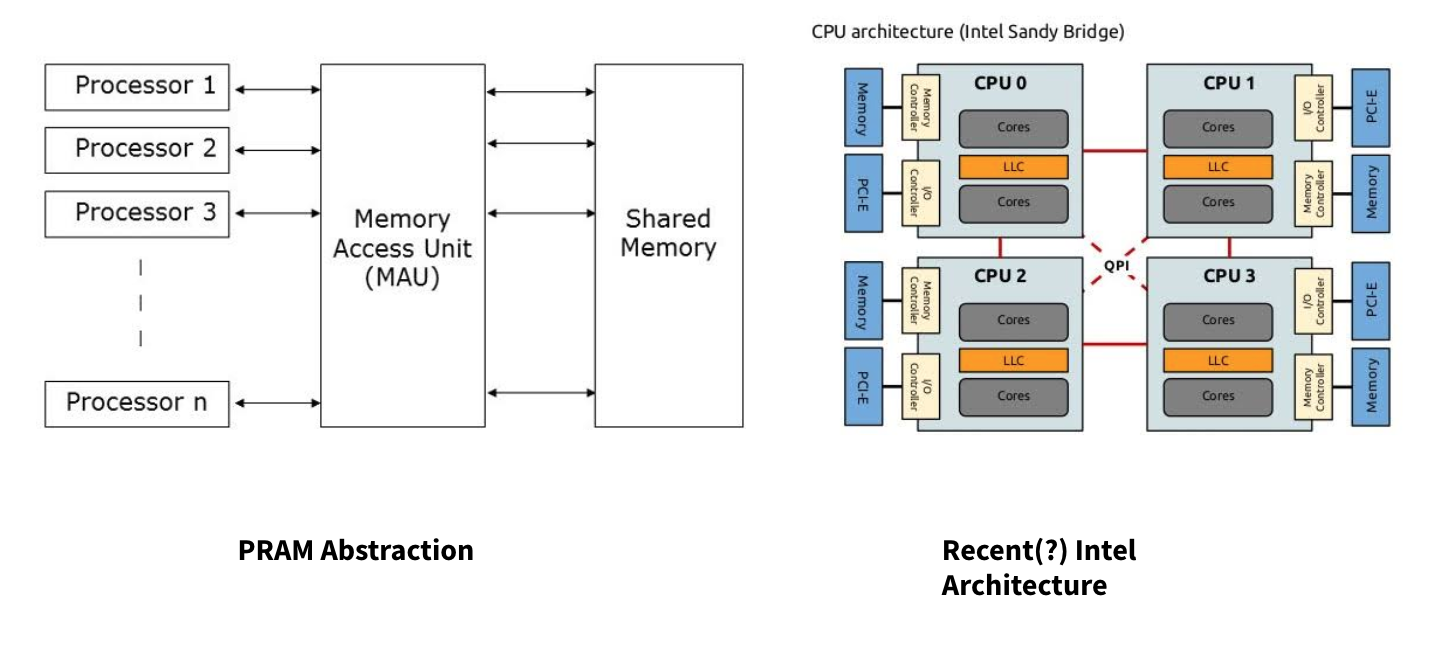
\includegraphics[scale=0.5]{parallel-architecture.png}
%   \caption{Splaying Example}
\end{figure}

\section{Nested Parallelism}
Nested parallel computations can be represented by dependency graphs (DAG). Two tasks are parallel if they are not reachable from each other.
\begin{figure}
  \centering
  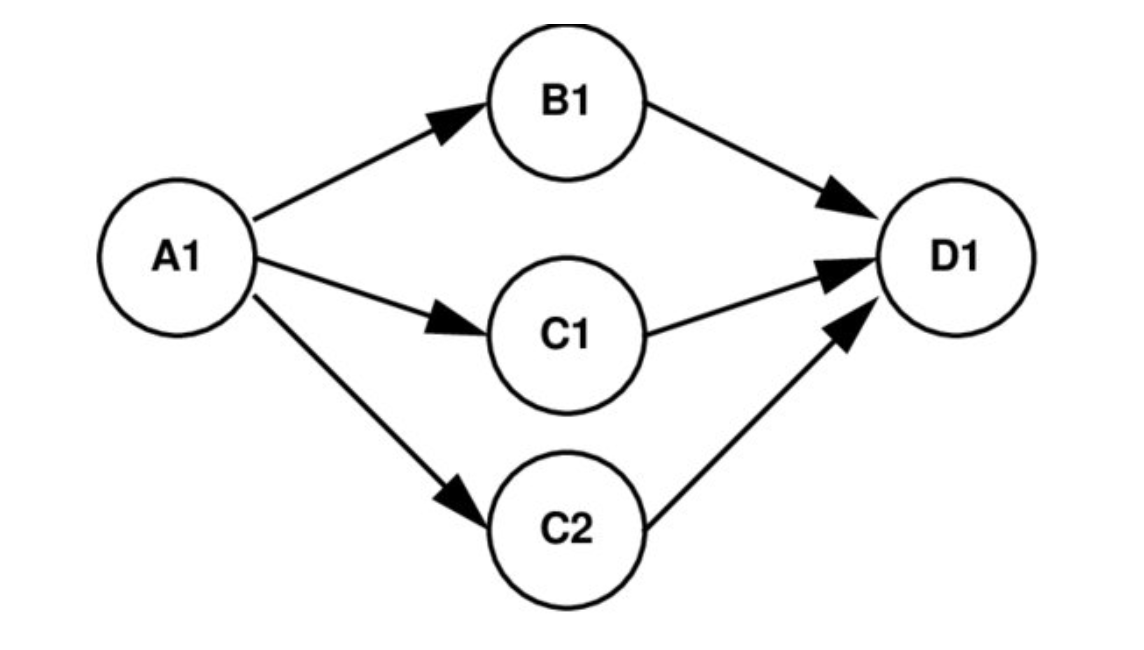
\includegraphics[scale=0.5]{dependency-graph.png}
   \caption{Dependency Graph}
\end{figure}
\begin{itemize}
    \item no synchronization among parallel tasks except at joint points
    \item Good schedulers are known
    \item Easy to understand, debug, and analyze
\end{itemize}

\subsection{Parallel For-Loop (pfor)}
Do these iterations in parallel. Usually accomplished by splitting the task into small pieces and running them simultaneously
\begin{figure}[h]
  \centering
  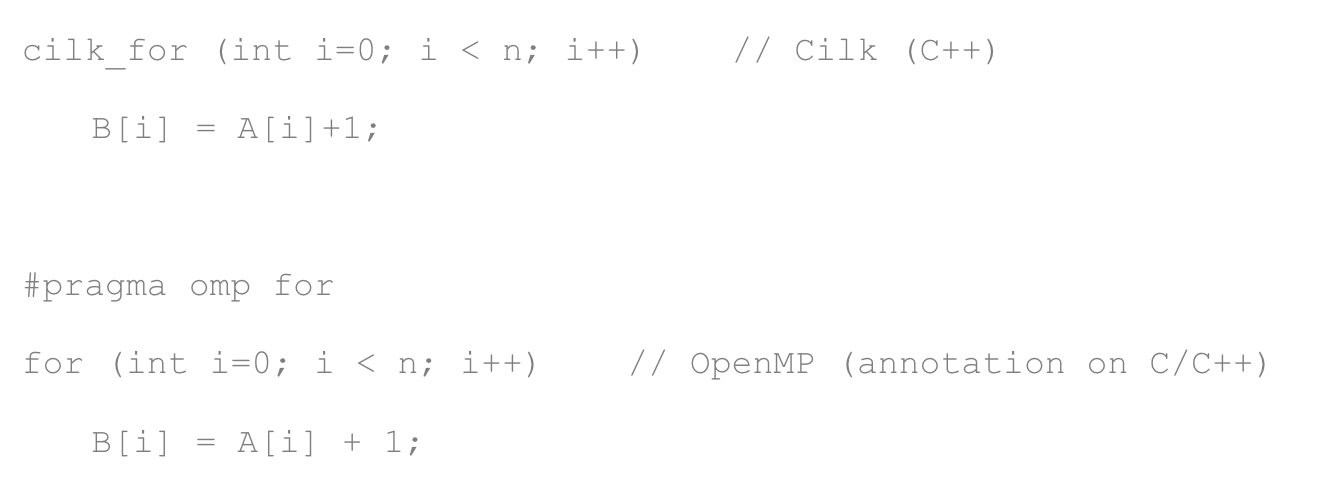
\includegraphics[scale=0.7]{cpp-pfor.png}
  \caption{Example of Parallel For-Loop in C++}
\end{figure}

\subsection{Fork-Join $(A \lvert\rvert B)$}
A way of setting up and executing parallel programs by "fork" execution branches off in parallel, then "join" to resume sequential execution. Parallel sections may fork recursively.
\begin{figure}
  \centering
  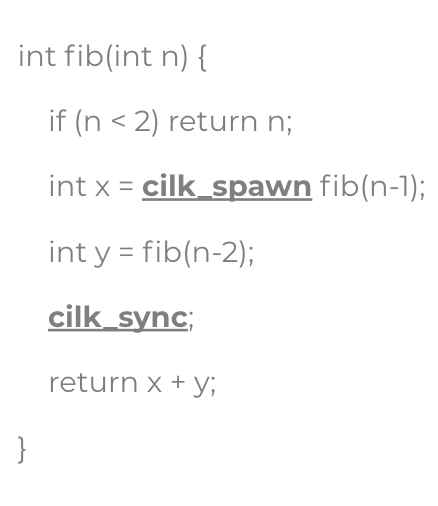
\includegraphics[scale=0.8]{cpp-forkjoin.png}
   \caption{Example of Fork-Join in C++}
\end{figure}

\subsection{Example in Pseudo-code}
\begin{figure}[H]
  \centering
  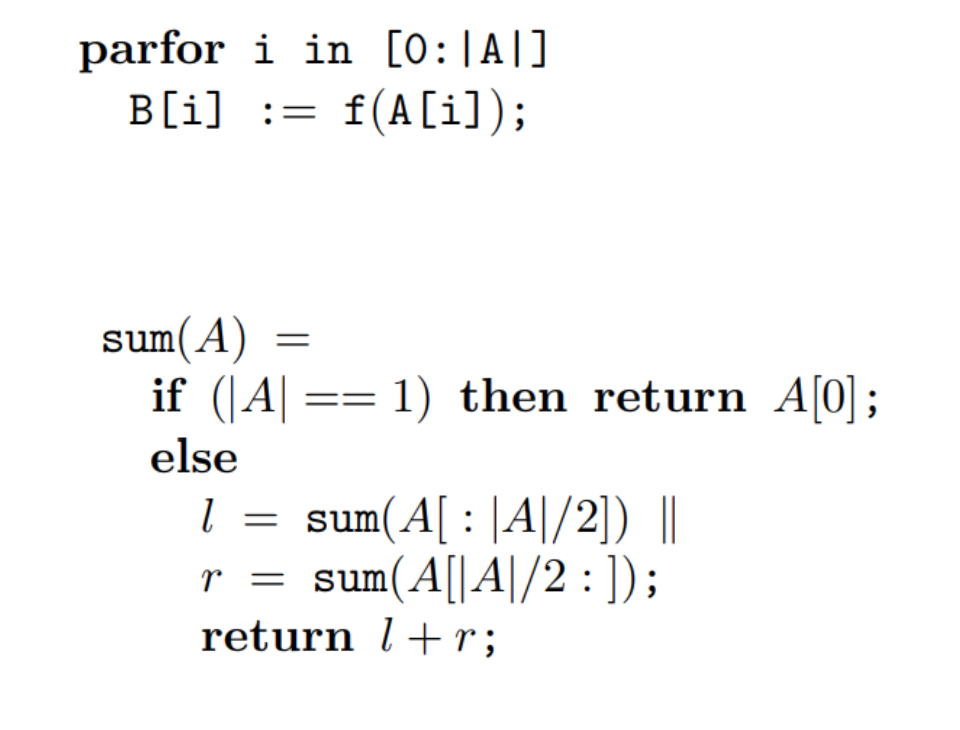
\includegraphics[scale=0.5]{pseudo-example.png}
\end{figure}

\section{Work/Depth Cost Model}
Work(W)
    $$W(n) := \text{total number of operations (costs are added across parallel calls)}$$
Span(S) or Depth(D)
$$S(n) := \text{depth/critical path of the computation (representing the longest chain of dependencies)}$$
Parallelism
$$\mathbb{P} = W/S$$

\subsection{Parallel For-Loop}
\begin{python}
pfor i in range(n):
    f(i)
\end{python}
Let $W_f(i)$ be work of $f(i)$ and $S_f(i)$ be span of $f(i)$
\begin{align*}
    W_{\text{total}} &= \sum_i^{n} W_f(i) \\
    S_{\text{total}} &= max_i S_f(i) 
\end{align*}

\subsection{Parallel Fork-Join}
\begin{python}
x,y = f(...) || g(...)
\end{python}
Let $W_f$ be work of f, $S_f$ be span of f, $W_g$ be work of g, and $S_g$ be span of g
\begin{align*}
    W_{\text{total}} &= W_f + W_g\\
    S_{\text{total}} &= max(S_f, S_g) 
\end{align*}

\subsection{Brent's Theorem}
Define
$$ T_p = \text{time on $p$ processors}$$
Let $W$ be total number of operations, $P$ be number of processors, and $S$ be sequential time steps
\begin{align*}
    T_p \leq \frac{W-S}{P} + S \\
    \intertext{in which}
    T_p \geq \frac{W-S}{P} \\
    \intertext{and}
    T_p \geq S
\end{align*}

\subsection{Goals}
\begin{enumerate}
    \item Work should be about the same as the sequential running time. When it matches asymptotically we say it is \textbf{work efficient}.
    \item Parallelism $(W/S)$ should be polynomial. $O(\sqrt{n})$ is probably good enough
\end{enumerate}

\section{Example: Sum}
Consider this implementation of $sum$
\begin{python}
def sum(xs):
    total = 0
    for i in xs:
        total += i
    return total
\end{python}
\begin{align*}
    W(n) &= O(n)\\
    S(n) &= O(n)
\end{align*}

If we change to use \textbf{pfor}, then
\begin{python}
def sum(xs):
    total = 0
    pfor i in xs:
        total += i
    return total
\end{python}
\begin{align*}
    W(n) &= O(n)\\
    S(n) &= O(1)
\end{align*}
However, we might encounter race condition, so discard this implementation\\
Recall the divide an conquer technique. If we halve the problem and recursively solve smaller problems in parallel (using fork-join).
\begin{python}
def sum_dq(xs):
    if len(xs) <= 1:
        return xs
    n = len(xs)
    l, r = sum_dq(xs[:n/2]) || sum_dq(xs[n/2:]
    return l+r
\end{python}
Assume that array slicing runs in $O(1)$ time by using pointers. Hence,
\begin{align*}
    W(n) &= 2W(n/2) + O(1) = O(n)\\
    S(n) &= S(n/2) + O(1) = O(logn)
\end{align*}

\section{QuickSort}
We will now see how can we make our beloved QuickSort parallel. Consider the following code :

\begin{python}
def qs(xs: Seq[Int]) -> Seq[Int]:
	if (len(xs) <= 1): return xs
	else:
		p = RNG.choice(xs)
		s0 = [ e for e in xs if e < p ]
		s1 = [ e for e in xs if e == p ] 
		s2 = [ e for e in xs if e > p ]
		(r0, r2) = par(qs(s0) || qs(s2))
		return r0 + s1 + r2
\end{python}

Lets analyze the time complexity of the parallel quick sort. By partition sequentially and appending in parallel, we then have work of $\O(n\log n)$ and span of $\O(n)$. Thus the parallelism, p, is $\frac{W}{S}=\O(\log n)$ which is not a very good parallelism.\\
\\
How can we have a better parallelism ?.
\subsection{Thought Experiment 1}

Assume: Partitioning and concatenation can be done in $\O(n)$ work and $\O(\log n)$ span but recursive calls are made sequentially.

\begin{figure}[h]
	\centering
	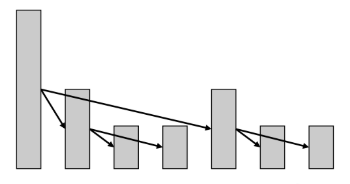
\includegraphics[scale=1]{qs-1.png}
	%   \caption{Splaying Example}
\end{figure}
What is the complexity of such assumption ? We have the work of $\O(n\log n)$ and span of $\O(n)$ therefore we get $\O(\log n)$ parallelism which is still not good enough.

\subsection{Thought Experiment 2}
Assume: Partitioning and concatenation can be done in $\O(n)$ work and $\O(log n)$ depth \textbf{and} recursive calls are made in parallel.

\begin{figure}[h]
	\centering
	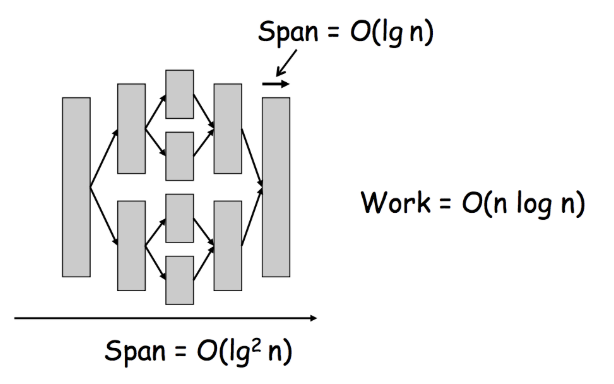
\includegraphics[scale=0.7]{qs-2.png}
	%   \caption{Splaying Example}
\end{figure}
Since for each concatenation, we have a span of $\O(\log n)$ hence overall span is of $\O(\log^2 n)$. The work of such assumption is $\O(n\log n)$ therefore we have the parallelism of $\O(n/\log n)$ which we consider a good parallel algorithm.

\section{Parallel Techniques}
Recall the following operations on collections :
\begin{enumerate}
	\item \lstinline|map|: applies a function $f$ to every element of the collection
	\item \lstinline|filter|: keep the element if element's predicate is true
	\item \lstinline|reduce|: pairwise combines elements in a tree until you have 1 using a (n associative) binary operator 
	\item etc
\end{enumerate}

\begin{tcolorbox}
	\textbf{Associative Binary Operator}
	\[ 
	\star: \U \times \U\mapsto \U
	\]
	eg. plus, multiply operator.\\
	
	The operator is said to be associative if $\forall a,b,c \in \U , (a\star b)\star c = a\star (b\star c)$
\end{tcolorbox}

\subsection{Map}
Consider the following parallel map algorithm:

\begin{python}
def par_map(xs: List[int], f: Callable) -> List[int]:
	out = []
	pfor i in range(n):
		out[i] = f(xs[i])
	return out
\end{python}

Hence we have $\O(n)$ work and $\O(1)$ span since we can apply $f$ to each element in parallel. Thus we have parallelism of $\O(n)$ 

\subsection{Reduce}

Define a reduce using associative binary operator above as follow:
\[
reduce(\star, xs) \mapsto x_1\star x_2 \dots \star x_n
\]
thus we can do $\star$ on all pairs first and then keep going down

\begin{align}
	\begin{forest}
	for tree={circle,draw, grow=north}
	[
	*
	[*
	[*[H][G]]
	[*[F][E]]
	]
	[*
	[*[D][C]]
	[*[B][A]]
	]
	]
	\end{forest}
\end{align}

Thus the number of elements each round are reduced by half. Hence we need to do $\O(\log n)$ round which make total work done be $\O(n)$ and $\O(\log n)$ span

\subsection{Filter}
A \lstinline|filter| takes input of collection $A$ and a predicate $p$ and return the collection containing $a \in A$ such that $p(a)$ is true in the same order as in $A$. Consider the following example:

Given a list $A=[2,1,4,0,3,1,5,7]$ with predicate $p(a): a<4$. We will perform the following step:
\begin{steps}
	\item{Compute the array of flag $F$, $F[i]=P(A[i])$\\ 
	Hence  we have $[1,1,0,1,1,1,0,0]$	
	}
\item {
	Apply \lstinline|plusScan| to the flag array $F$ and maps to the indexes array, $I$. \\
	Hence we have $[0,1,2,2,3,4,5,5]$
}
\item {
	Now we allocate result array, $R$ where $R[i] = X[I[i]]$.\\
	Thus we have the final result $[2,1,0,3,1]$
}
\end{steps}

Thus we have a total work for \lstinline|filter| of $\O(n)$ and span of $\O(\log n)$ from \lstinline|plusScan|

\subsection{Flatten}
The \lstinline|flatten| takes a nested sequence $A$ as input and return a flatten sequence $R$ that contains each sequences in $A$ concatenate together.\\
For example, \lstinline|flatten([[3,2], [2,3,4],[5],[1,2,7,9]]) = [3,2,2,3,4,5,1,2,7,9]|
%Finally, if you have citations, see the commented-out stuff in the \LaTeX~here.

%\

%My farourive Optimization books are \cite{bertsimas1997introduction} \cite{boyd2004convex} \cite{wolsey2014integer}. You should add bibliographical notes in the \textbf{BibTex}: \textit{mybib.bib} file. Its good to grab these notes from Google scholar citations.

%%%%%%%%%% If you don't have citations then comment the lines below:

%\bibliographystyle{abbrv}           % if you need a bibliography
%\bibliography{mybib}                % assuming yours is named mybib.bib


%%%%%%%%%%% end of doc
\end{document}

